\chapter{Aspectos Conceituais}
\label{cap:astronomia}



\begin{overview}
  \lipsum[1]
\end{overview}


\section{Astrometria}
\label{sec:astrometria}

Astrometria é uma disciplina da astronomia responsável pela medição precisa das posições, distâncias e movimentos dos corpos celestes, essencial para a construção e manutenção de catálogos astronômicos. Esta área fundamenta-se em técnicas observacionais que visam determinar coordenadas angulares relativas a sistemas de referência celestes. Nesta seção, serão abordados alguns conceitos fundamentais de astronomia para o desenvolvimento deste projeto, como sistema de coordenadas (Seção \ref{sec:sistema-coordenadas}) e brilho (Seção \ref{sec:magnitude}).

\subsection{Sistema de Coordenadas}
\label{sec:sistema-coordenadas}

\begin{figure}[!ht]
  \centering
  \caption{Sistema de coordenadas equatorial}
  \label{fig:sistema-equatorial}
  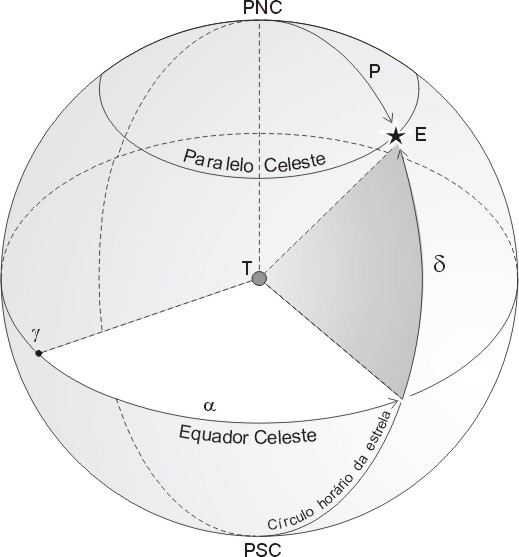
\includegraphics[width=0.58\linewidth]{figures/coords.png}
  \fonte{Núcleo Olímpico de Incentivo ao Conhecimento (NOIC). Disponível em: \url{https://noic.com.br/coordenadas-celestes}}
\end{figure}

Diversos sistemas de coordenadas são usados na astronomia, como o azimutal, o eclíptico e o equatorial. Esse último é amplamente usado na astronomia e o padrão em levantamentos astronômicos digitais (Seção \ref{sec:surveys}) sendo adotado como padrão nesse trabalho, tanto em tabelas quanto em figuras.

O sistema equatorial é composto pelas coordenadas de ascensão reta ($\alpha$ ou RA) e declinação ($\delta$ ou Dec). A ascensão reta é análoga à longitude e é medida em horas, minutos e segundos, ao longo do equador celeste, a partir do ponto vernal ($\gamma$), que é o ponto onde o Sol cruza o equador celeste na direção do hemisfério celestial norte durante o equinócio de março. A declinação, semelhante à latitude, é medida em graus acima ou abaixo do equador celeste, variando de $+90^{\circ}$ no polo celeste norte a $-90^{\circ}$ no polo celeste sul. A Fig. \ref{fig:sistema-equatorial} mostra um esquema do sistema equatorial. Nela, o ponto $E$, marcado com uma estrela, representa um objeto celeste (ou astro) e pode ser definido pelo par de coordenadas $E = (\alpha, \delta)$.

Esse sistema de coordenadas é fundamental para a localização de objetos no céu e baseia-se no conceito da esfera celeste. A esfera celeste é uma representação imaginária do céu, uma superfície esférica de grande raio centrada na Terra (representada como o ponto T na Fig. \ref{fig:sistema-equatorial}), sobre a qual todos os objetos astronômicos parecem estar fixados. Essa concepção é útil porque facilita a definição de coordenadas angulares para descrever a posição de objetos no céu, similar ao sistema de latitude e longitude empregado na superfície terrestre. A esfera celeste é dividida por planos de referência como o equador celeste, que é a projeção do equador terrestre, e o eixo de rotação da Terra, que define os polos celestes norte (PNC) e sul (PSC).

% A utilização da esfera celeste e das coordenadas equatoriais tem implicações significativas para as estruturas de dados empregadas em grandes catálogos astronômicos. Na próxima subseção, será discutido como explorar o conceito da esfera celeste para definir uma técnica eficiente de armazenamento e busca de objetos astronômicos.

% Dado o gigantesco volume de dados gerados por levantamentos astronômicos, é necessário desenvolver métodos eficientes para armazenar, processar e recuperar informações de forma precisa e rápida. Estruturas de dados específicas, como árvores de espaço de varredura (sky partitioning trees), k-d trees \cite{kdtree} e algoritmos baseados em hierarquias de pixels, como o sistema HEALPix \cite{healpix} e HIPS \cite{hips}, são amplamente utilizadas para indexar as posições dos objetos na esfera celeste. Essas estruturas permitem a divisão da esfera celeste em regiões menores e hierarquicamente organizadas, facilitando buscas eficientes e operações de vizinhança, que são essenciais em tarefas como a identificação de aglomerados de galáxias ou a execução de cruzamentos de dados entre diferentes levantamentos. Esse assunto será abordado com mais detalhes na próxima subseção.

% A representação esférica e as coordenadas angulares também impactam a precisão e a complexidade computacional dos algoritmos utilizados. Transformações de coordenadas, cálculos de distância angular e correções devido a efeitos astronômicos, como a aberração e a refração, devem ser tratados adequadamente para garantir a precisão dos dados astronômicos. Assim, a gestão de grandes catálogos astronômicos exige não apenas estratégias de armazenamento eficiente, mas também métodos robustos para garantir que as consultas e análises mantenham a precisão necessária para os estudos científicos que dependem desses dados.




\subsection{Brilho e Magnitude}
\label{sec:magnitude}

O brilho e a magnitude são conceitos fundamentais para quantificar a intensidade de luz emitida ou refletida por objetos celestes, sendo essenciais para a caracterização de estrelas, galáxias e outros corpos celestes. O brilho refere-se à quantidade total de energia luminosa recebida por unidade de área em um detector, como um telescópio. É uma medida física direta da intensidade de luz e varia inversamente com o quadrado da distância do objeto, sendo comumente expresso em termos de fluxo, que é a quantidade de luz recebida por unidade de área por unidade de tempo. A medição do brilho permite aos astrônomos determinar características intrínsecas dos objetos, como temperatura e tamanho, e é um dos parâmetros centrais para estudar a evolução estelar e a estrutura galática.

A magnitude, por outro lado, é uma medida que descreve o brilho percebido dos objetos astronômicos em escala logarítmica, introduzida para lidar com a vasta gama de intensidades luminosas observadas no céu. A escala de magnitude é inversa, de forma que objetos mais brilhantes têm magnitudes menores, enquanto objetos mais fracos têm magnitudes maiores. A magnitude aparente quantifica o brilho de um objeto visto da Terra, enquanto a magnitude absoluta define o brilho que o objeto teria se estivesse a uma distância padrão de 10 parsecs. Essa distinção permite a comparação do brilho intrínseco de diferentes objetos, independentemente de sua distância da Terra.






\section{Parâmetros Geométricos das Galáxias}
\label{sec:parametros-geometricos}


\subsection{Raio Efetivo}
\label{sec:raio-efetivo}

O raio efetivo de uma galáxia é uma medida fundamental em astronomia que caracteriza a distribuição espacial de sua luminosidade. Em termos práticos, o raio efetivo é definido como a distância do centro da galáxia até o ponto onde metade da luz total emitida galáxia está concentrada. Essa métrica é amplamente utilizada para descrever a extensão aparente das galáxias e fornece informações valiosas sobre sua estrutura interna e dinâmica.

O cálculo do raio efetivo depende da análise da distribuição de brilho da galáxia, sendo comumente obtido por meio de perfis de brilho de superfície que representam a intensidade luminosa em função da distância ao centro da galáxia. Para galáxias elípticas, esses perfis de brilho são tipicamente modelados por uma distribuição de Sérsic, que se ajusta bem à sua estrutura concentrada. Já para galáxias espirais, a distribuição de brilho tende a ser mais complexa, com um núcleo brilhante e uma extensão de braços espirais, o que pode exigir ajustes mais detalhados para determinar o raio efetivo.

\subsection{Elipticidade}
\label{sec:elipticidade}

A elipticidade complexa é uma métrica amplamente utilizada em estudos de lentes gravitacionais, onde se faz necessária a quantificação precisa da distorção observada nas imagens de objetos distantes devido à ação gravitacional de um objeto massivo interveniente, como uma galáxia ou um aglomerado de galáxias. Essa métrica é essencial para descrever a forma das imagens distorcidas, permitindo a análise da distribuição de massa do objeto que atua como lente. Especificamente, a elipticidade complexa captura a deformação das fontes de luz distantes sob a forma de uma componente elíptica, expressando tanto a intensidade da distorção (ou seja, o alongamento da imagem) quanto a sua orientação no plano do céu.

A métrica de elipticidade complexa é particularmente útil na modelagem e análise de lentes fracas, em que as distorções são sutis e a forma das galáxias de fundo serve como uma sonda estatística para inferir a presença de matéria escura e a estrutura da lente gravitacional. Essa métrica desempenha um papel crucial para estudos que investigam a distribuição de matéria escura e a formação de grandes estruturas no universo. Ao quantificar a distorção induzida por lentes gravitacionais, os astrônomos podem mapear a distribuição de massa em escalas cósmicas, incluindo matéria que não emite luz visível, como a matéria escura. Em estudos de lenteamento fraco, onde os efeitos de distorção são mínimos e requerem uma análise estatística sobre grandes populações de galáxias, a elipticidade complexa oferece uma forma consistente e precisa de capturar e interpretar essas pequenas distorções.







\section{Levantamentos Astronômicos}
\label{sec:surveys}
Um levantamento astronômico consiste em uma pesquisa sistemática de grandes áreas do céu com o intuito de coletar dados sobre objetos e fenômenos celestes \cite[p. 40-42]{extragalactic-astronomy-book}. Estes levantamentos abrangem observações em diferentes faixas do espectro eletromagnético e buscam identificar e catalogar astros como estrelas, galáxias, aglomerados e nebulosas, fornecendo uma base de dados ampla e acessível para estudos detalhados \cite{astronomical-survey}. A finalidade dos levantamentos é construir um mapa celeste que permita compreender a distribuição e as propriedades dos corpos celestes em diversas escalas, auxiliando na análise estatística de populações estelares e galácticas e na identificação de estruturas de larga escala, como filamentos e vazios cósmicos \cite{bahcall1995,baleisis1998,jarrett2004}.

O grande volume de dados gerado por esses levantamentos astronômicos representa um desafio significativo. Os avanços em tecnologia de sensoriamento e armazenamento permitiram que telescópios modernos capturassem bilhões de objetos celestes em detalhes, gerando petabytes de dados que precisam ser processados, organizados e armazenados \cite{szalay2000,graefe1993}. Este volume de dados impõe desafios em termos de infraestrutura de armazenamento, processamento e análise, além de exigir métodos eficientes de organização e recuperação de informações. Para enfrentar esses desafios, foram desenvolvidos os chamados observatórios virtuais \cite{ivoa}, que integram e centralizam os dados provenientes de diversos levantamentos. Estes observatórios permitem o acesso distribuído aos dados e promovem a interoperabilidade entre diferentes conjuntos de dados, facilitando a análise conjunta de observações realizadas em diferentes regiões do espectro e por distintos instrumentos \cite{sciserver}.

A existência de múltiplos levantamentos astronômicos fotométricos se justifica pela necessidade de observar o universo em diferentes comprimentos de onda, uma vez que cada faixa do espectro revela características específicas dos objetos astronômicos. Por exemplo, a radiação ultravioleta é útil para identificar regiões de formação estelar intensa, enquanto o infravermelho é empregado na observação de regiões obscurecidas por poeira interestelar \cite[p. 28-31]{extragalactic-astronomy-book}. Assim, levantamentos em faixas distintas do espectro eletromagnético fornecem dados complementares que permitem uma visão mais completa dos processos físicos no cosmos. A variabilidade na profundidade (capacidade de observar objetos mais distantes e fracos) e na resolução espacial também diversifica os objetivos dos levantamentos. Nas próximas subseções, serão apresentadas breves descrições dos levantamentos utilizados no desenvolvimento deste projeto.







\subsection{Galaxy Evolution Explorer}
\label{sec:galex}

O Galaxy Evolution Explorer (GALEX) foi um telescópio espacial da NASA dedicado a levantamentos astronômicos no ultravioleta (UV), operando entre 2003 e 2013. Como observatório orbital, evitou a absorção atmosférica terrestre, permitindo imageamento e espectroscopia de alta sensibilidade em duas bandas: FUV (1350--1780 \AA) e NUV (1770--2830 \AA). Sua cobertura espacial alcançou $\approx$26.000 graus quadrados ($\approx$63\% do céu), incluindo áreas profundas (múltiplas exposições) e extensas (varreduras rasas), com resolução angular de 1.2--1.5 arcsec.

\begin{figure}[!ht]
  \centering
  \caption{Cobertura espacial e espectral do levantamento Galex}
  \label{fig:galex}
  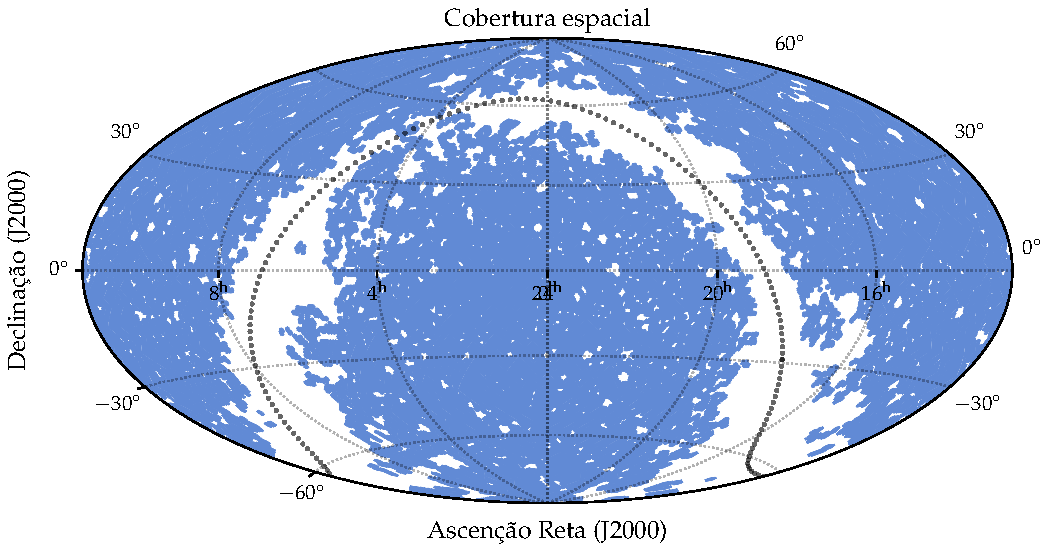
\includegraphics[width=0.61\linewidth]{figures/footprint_galex.pdf}\hfill
  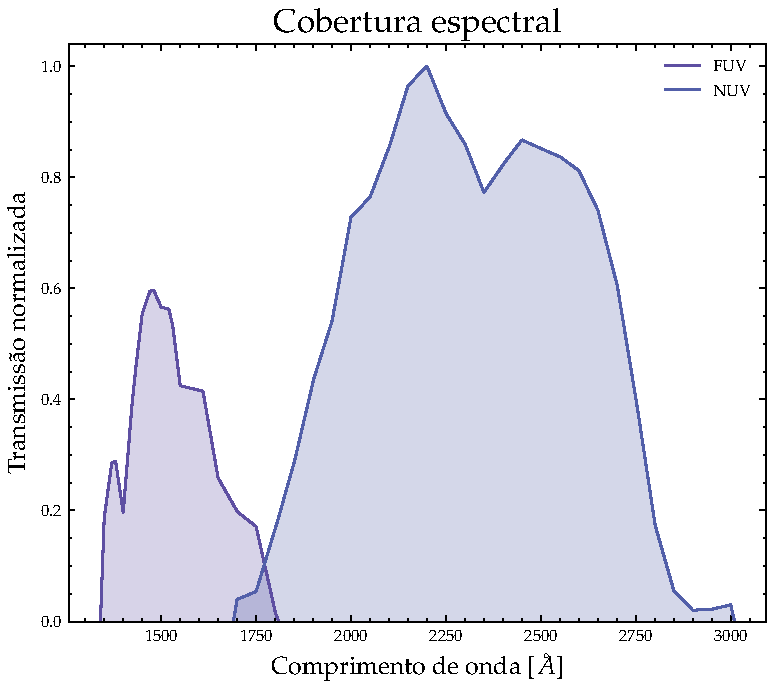
\includegraphics[width=0.37\linewidth]{figures/transmission_galex.pdf}
  \legend{A área de cobertura espacial do levantamento é mostrada no painel à esquerda na região em azul. A corbertura espectral é mostrada no painel à direita com as curvas de transmissão total dos dois filtros NUV e FUV em função do comprimento de onda.}
\end{figure}





\subsection{Southern Photometric Local Universe Survey}
\label{sec:splus}

\begin{figure}[!ht]
  \centering
  \caption{Cobertura espacial e espectral do levantamento S-PLUS}
  \label{fig:splus}
  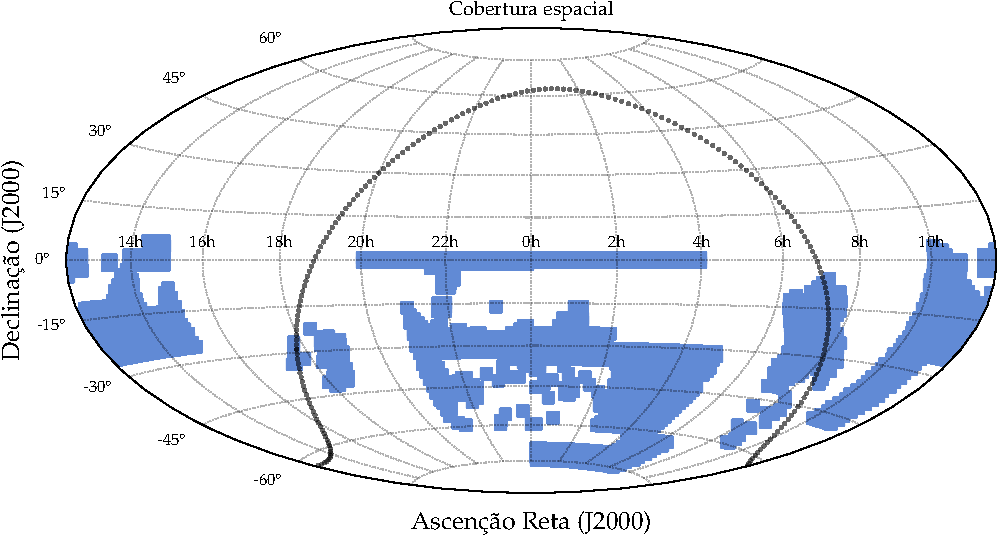
\includegraphics[width=0.61\linewidth]{notebooks/plots/footprint_splus.pdf}\hfill
  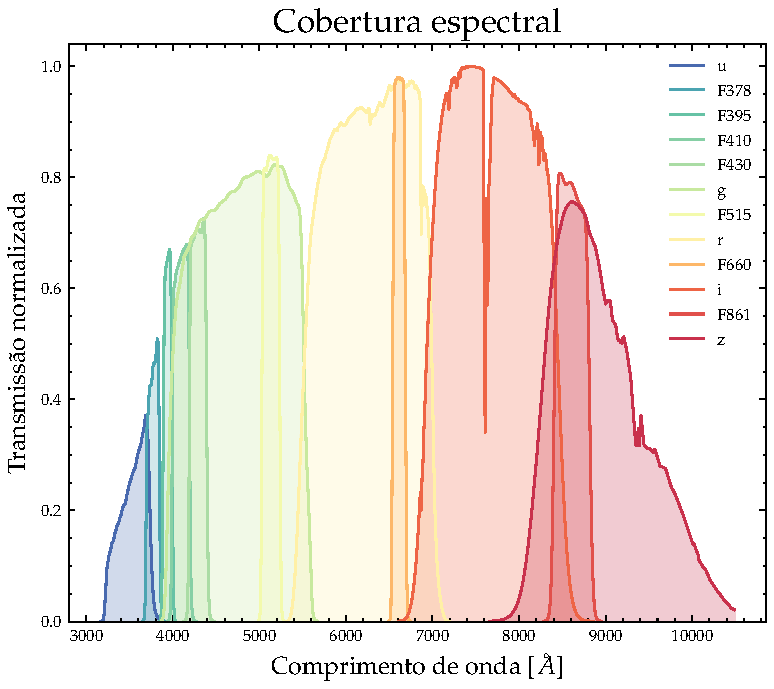
\includegraphics[width=0.37\linewidth]{figures/transmission_splus.pdf}
  \legend{A área de cobertura espacial do levantamento é mostrada no painel à esquerda na região em azul. A corbertura espectral é mostrada no painel à direita com as curvas de transmissão total dos quatro filtros g, r, i e z em função do comprimento de onda.}
\end{figure}

O levantamento astronômico brasileiro Southern Photometric Local Universe Survey\footnote{\url{https://splus.iag.usp.br}} (S-PLUS; \citealp{splus}) é um mapeamento do hemisfério celestial sul utilizando uma abordagem multibanda altamente detalhada. O S-PLUS utiliza o telescópio T80-Sul, localizado no Observatório de Cerro Tololo, no Chile, para observar uma área de aproximadamente 8.000 graus quadrados, como mostra a Fig. \ref{fig:splus}.

Um dos principais diferenciais do S-PLUS é a sua cobertura em doze bandas fotométricas, que incluem cinco bandas similares às do levantamento SDSS (u, g, r, i, z) e sete bandas estreitas (J0378, J0395, J0410, J0430, J0515, J0660, J0861) com comprimentos de onda variando entre 3780 \AA e 8610 \AA. Essa configuração de bandas permite uma análise espectral rica, capturando detalhes como a presença de linhas de emissão e absorção específicas, que são cruciais para a determinação precisa de parâmetros físicos e químicos dos objetos observados. Por exemplo, as bandas estreitas foram escolhidas para registrar características específicas como o traço do cálcio, magnésio e oxigênio, o que facilita a análise da composição estelar e a identificação de processos de formação estelar. Seus dados são disponibilizados pela plataforma S-PLUS Cloud (\url{https://splus.cloud}).






\subsection{Legacy Surveys}
\label{sec:legacy}

\begin{figure}[!ht]
  \centering
  \caption{Cobertura espacial e espectral do levantamento Legacy}
  \label{fig:legacy}
  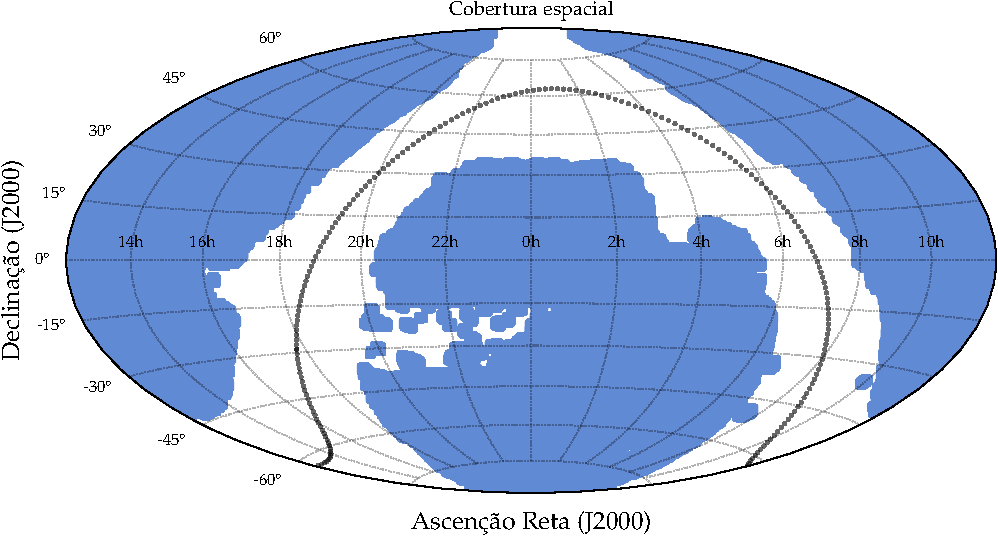
\includegraphics[width=0.61\linewidth]{notebooks/plots/footprint_legacy.pdf}\hfill
  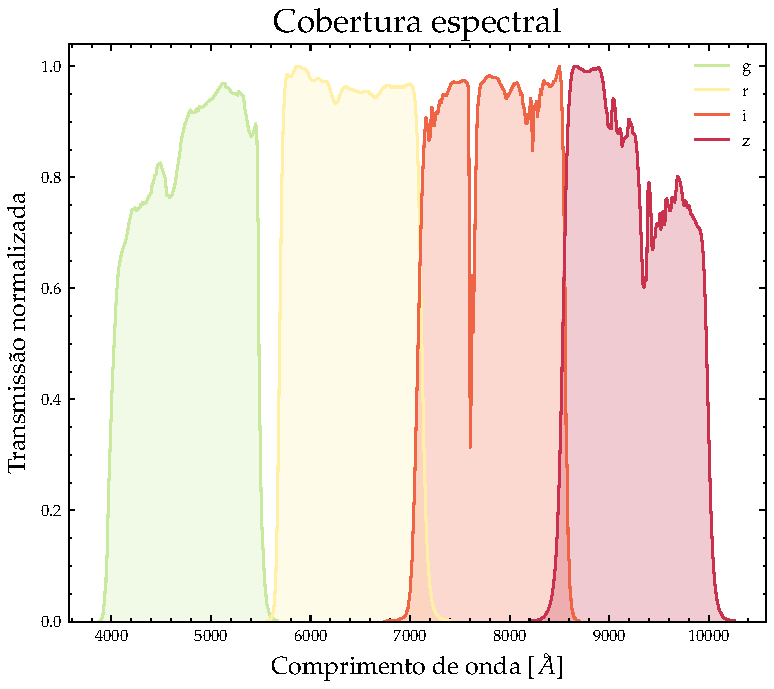
\includegraphics[width=0.37\linewidth]{figures/transmission_legacy.pdf}
  \legend{A área de cobertura espacial do levantamento é mostrada no painel à esquerda na região em azul. A corbertura espectral é mostrada no painel à direita com as curvas de transmissão total dos quatro filtros g, r, i e z em função do comprimento de onda.}
\end{figure}

Os Legacy Surveys\footnote{\url{https://legacysurvey.org}} \cite{legacy} consistem em três projetos individuais e complementares: o Dark Energy Camera Legacy Survey (DECaLS), o Beijing-Arizona Sky Survey (BASS) e o Mayall z-band Legacy Survey (MzLS). Juntos, formam um dos maiores projetos de mapeamento digital do céu, projetado para fornecer uma base fotométrica abrangente para o projeto Dark Energy Spectroscopic Instrument (DESI). O Legacy Survey cobre aproximadamente 14.000 graus quadrados do céu. Esse levantamento oferece uma cobertura profunda e em múltiplas bandas fotométricas, incluindo as bandas $g$, $r$, $i$ e $z$, com comprimentos de onda centrados em aproximadamente 4750 \AA, 6300 \AA, 7800 \AA e 9200 \AA, respectivamente. Essas bandas, juntamente com sua grande profundidade, permitem a detecção de objetos mais fracos e distantes, possibilitando estudos detalhados da distribuição de galáxias e outras estruturas em grandes escalas.

A profundidade dos Legacy Surveys é um dos fatores que o diferencia de outros levantamentos. Com exposições projetadas para alcançar uma profundidade mais elevada, os Legacy Surveys são capazes de detectar objetos com brilho mais tênue, o que é fundamental para o mapeamento detalhado da estrutura de larga escala do universo.
%Este aspecto é essencial para o projeto DESI, que utiliza os dados do Legacy Survey para selecionar alvos para espectroscopia, a fim de estudar a energia escura e a expansão cósmica. 









\subsection{UKIRT Infrared Deep Sky Survey}
\label{sec:dados-ukidss}

O UKIRT Infrared Deep Sky Survey (UKIDSS) é um levantamento conduzido pelo telescópio terrestre United Kingdom Infrared Telescope (UKIRT) no Havaí, operando exclusivamente no infravermelho próximo. Sua cobertura espacial é de, aproximadamente, 7.500 graus quadrados do céu norte. As observações são feitas em cinco bandas fotométricas: Z (8800 \AA), Y (10300 \AA), J (12500 \AA), H (16300 \AA) e K (22000 \AA), com resolução angular de $\approx$0,8 arcseg (FWHM) e profundidade típica de K $\approx$ 18,2 mag.

\begin{figure}[!ht]
  \centering
  \caption{Cobertura espacial e espectral do levantamento UKIDSS}
  \label{fig:footprint-ukidss}
  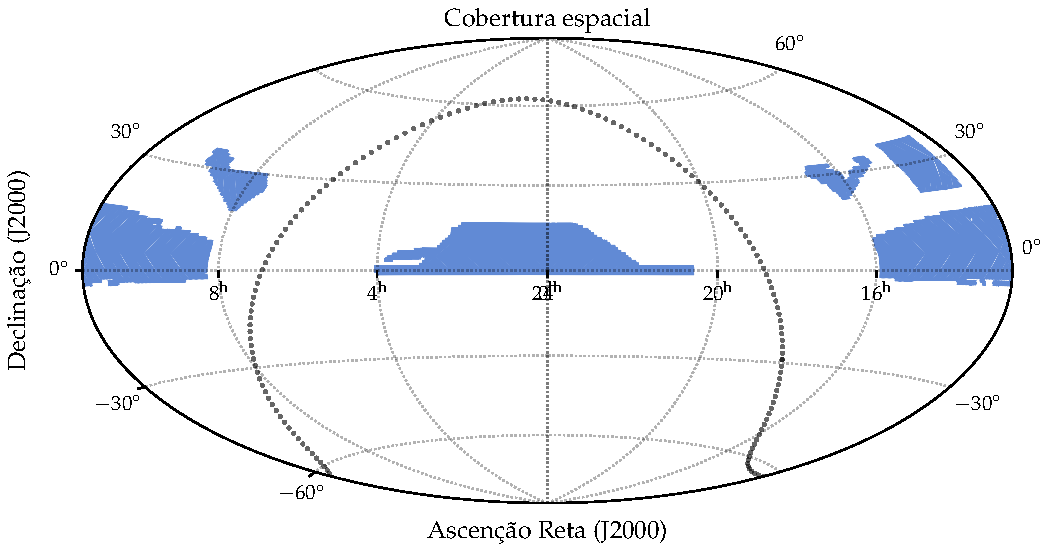
\includegraphics[width=0.61\linewidth]{figures/footprint_ukidss.pdf}\hfill
  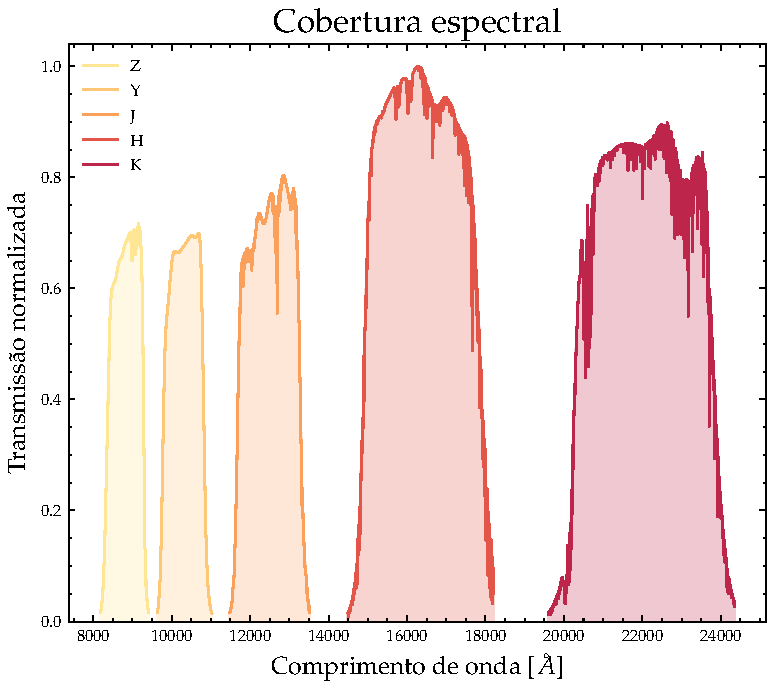
\includegraphics[width=0.37\linewidth]{figures/transmission_ukidss.pdf}
  \legend{A área de cobertura espacial do levantamento é mostrada no painel à esquerda na região em azul. A corbertura espectral é mostrada no painel à direita com as curvas de transmissão total dos cinco filtros Z, Y, J, H e K em função do comprimento de onda.}
\end{figure}






\subsection{Vista Hemisphere Survey}
\label{sec:vista}

O Vista Hemisphere Survey (VHS) é um levantamento astronômico terrestre conduzido pelo telescópio VISTA (Visible and Infrared Survey Telescope for Astronomy) no Observatório do Paranal (Chile). Opera exclusivamente no infravermelho próximo (IR), abrangendo 20.000 graus quadrados do hemisfério sul celeste (declinação $< +0.5^\circ$), incluindo regiões de alta densidade estelar como o Plano Galático. Utiliza a câmera VIRCAM com cinco bandas fotométricas: Z (8800 \AA), Y (10200 \AA), J (12500 \AA), H (16500 \AA) e Ks (21500 \AA), alcançando resolução angular de 0.34 arcsec/pixel e profundidade típica de Ks $\approx$ 18 mag.

\begin{figure}[!ht]
  \centering
  \caption{Cobertura espacial e espectral do levantamento VHS}
  \label{fig:footprint-vhs}
  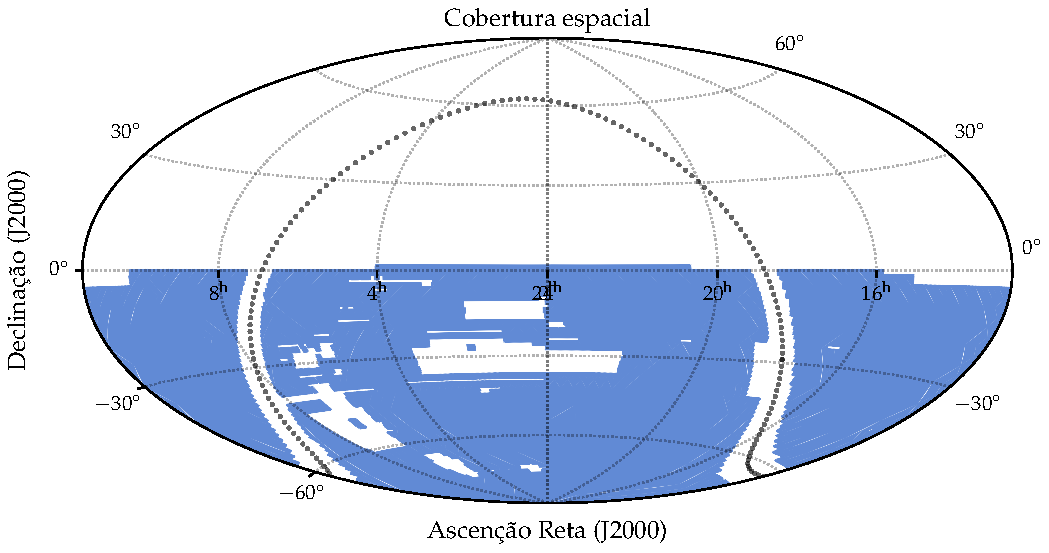
\includegraphics[width=0.61\linewidth]{figures/footprint_vista.pdf}\hfill
  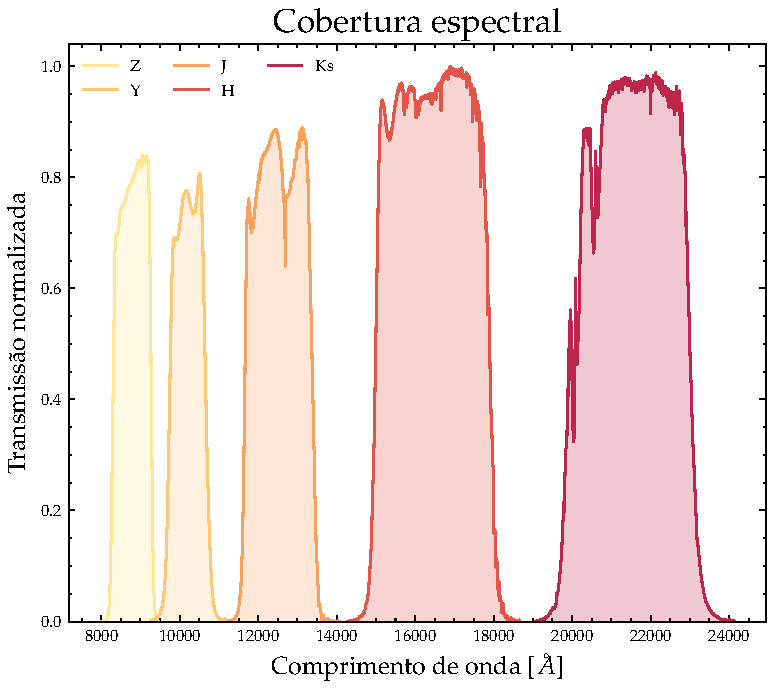
\includegraphics[width=0.37\linewidth]{figures/transmission_vista.pdf}
  \legend{A área de cobertura espacial do levantamento é mostrada no painel à esquerda na região em azul. A corbertura espectral é mostrada no painel à direita com as curvas de transmissão total dos cinco filtros Z, Y, J, H e Ks em função do comprimento de onda.}
\end{figure}







\subsection{Wide-field Infrared Survey Explorer}
\label{sec:unwise}

O Wide-field Infrared Survey Explorer (WISE) é um telescópio espacial da NASA que realizou um levantamento \emph{all-sky} em quatro bandas do infravermelho médio: W1 (34000 \AA), W2 (46000 \AA), W3 (120000 \AA) e W4 (220000 \AA), com resolução angular de 6.1 arcsec, 6.4 arcsec, 6.5 arcsec e 12.0 arcsec respectivamente. Cobrindo 100\% do céu com múltiplas varreduras, gerou um catálogo de mais de 750 milhões de fontes, utilizando detectores HgCdTe resfriados criogenicamente (operando a 17K) para minimizar ruído térmico. A missão primária (2010) mapeou o céu completo uma vez e meia, enquanto a extensão NEOWISE (2013-presente) continua monitoragem nas bandas W1 e W2.

\begin{figure}[!ht]
  \centering
  \caption{Cobertura espacial e espectral do levantamento WISE}
  \label{fig:footprint-unwise}
  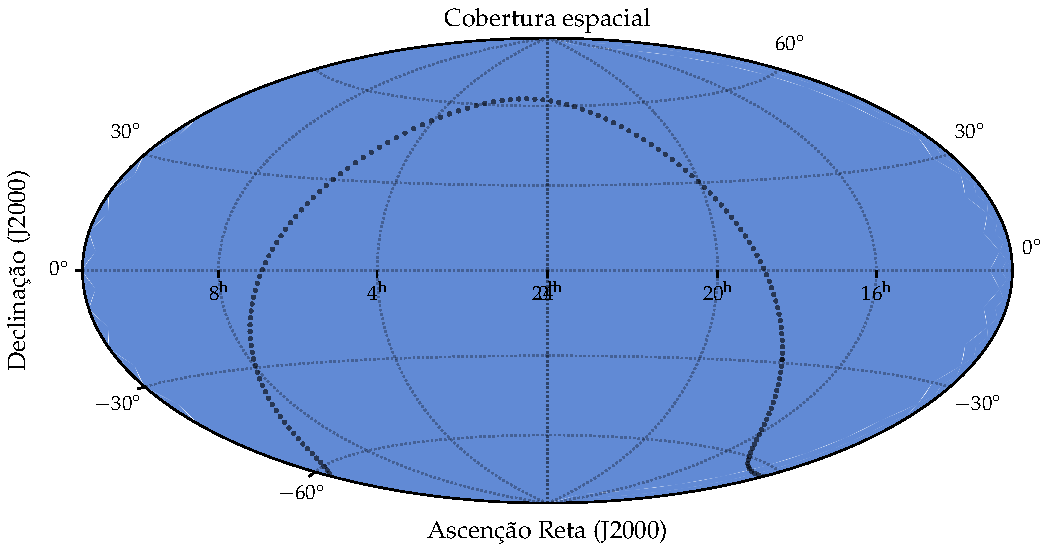
\includegraphics[width=0.61\linewidth]{figures/footprint_unwise.pdf}\hfill
  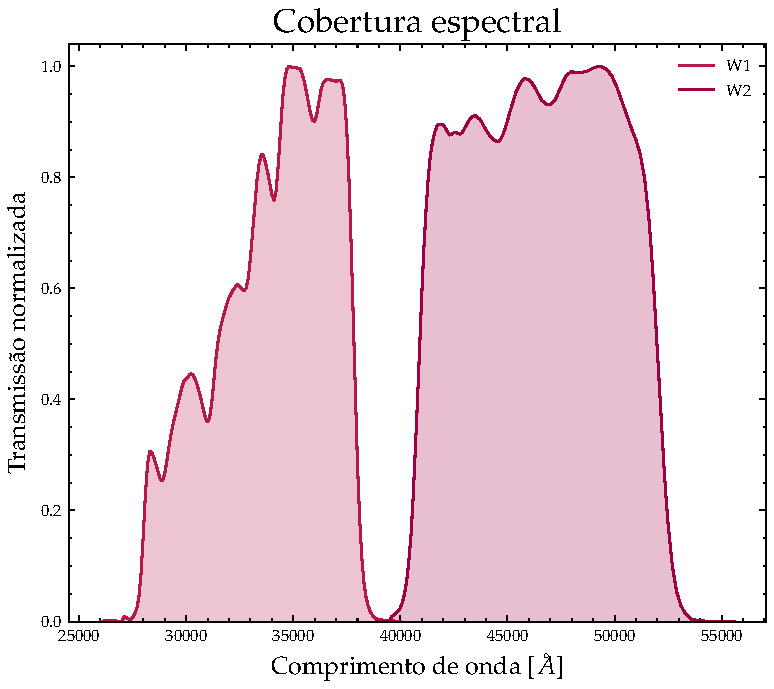
\includegraphics[width=0.37\linewidth]{figures/transmission_unwise.pdf}
  \legend{A área de cobertura espacial do levantamento é mostrada no painel à esquerda na região em azul. A corbertura espectral é mostrada no painel à direita com as curvas de transmissão total dos dois filtros W1 e W2 em função do comprimento de onda.}
\end{figure}








% \subsection{Sloan Digital Sky Survey}
% \label{sec:sdss}

% \begin{figure}[!ht]
%   \caption{Área de cobertura do levantamento SDSS}
%   \label{fig:coverage-sdss}
%   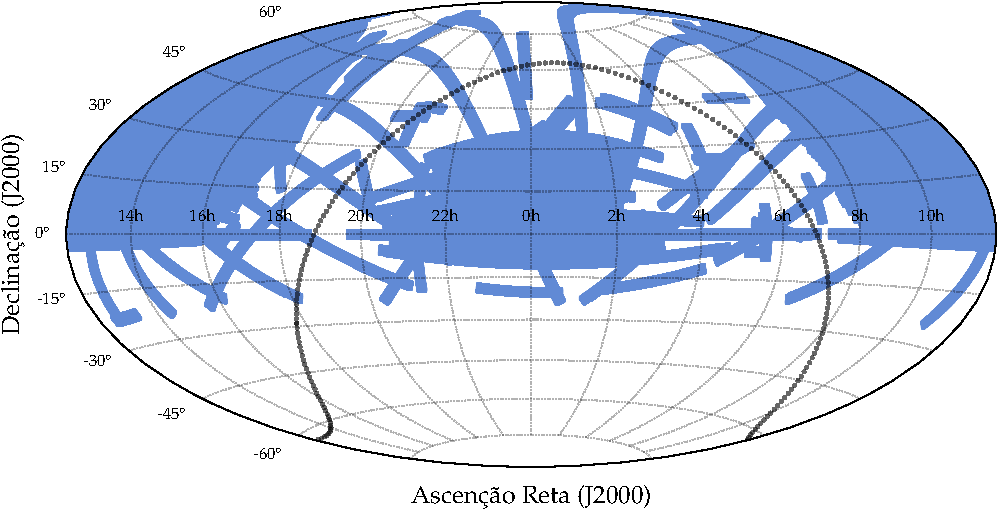
\includegraphics[width=\linewidth]{notebooks/plots/sdss_footprint.pdf}
% \end{figure}

% O Sloan Digital Sky Survey\footnote{\url{https://sdss.org}} (SDSS; \citealp{sdss}) é um dos levantamentos astronômicos mais influentes e abrangentes, sendo pioneiro no uso de técnicas digitais para mapear o céu noturno. Iniciado em 2000, o SDSS empregou um telescópio dedicado de 2,5 metros \cite{sdss-telescope} equipado com uma poderosa câmera de dispositivo de carga acoplada (CCD;  \citealp{sdss-camera}) para mapear o céu do norte com detalhes sem precedentes, cobrindo uma área de cerca de 14.000 graus quadrados, principalmente no hemisfério celestial norte. A Fig. \ref{fig:coverage-sdss} mostra a área de cobertuda da décima oitava liberação de dados (DR18; \citealp{sdss-dr18}). Ao longo de suas diferentes fases, o levantamento produziu dados detalhados de milhões de estrelas, galáxias e quasares, contribuindo significativamente para o avanço de áreas como cosmologia, formação de galáxias e estrutura de larga escala do universo.

% O SDSS foi um dos primeiros levantamentos a realizar observações em múltiplas bandas fotométricas, abrangendo cinco faixas do espectro eletromagnético: u, g, r, i e z \cite{sdss-filters}, com comprimentos de onda centrados em 3543 $\si{\angstrom}$, 4770 $\si{\angstrom}$, 6231 $\si{\angstrom}$, 7625 $\si{\angstrom}$ e 9134 $\si{\angstrom}$, respectivamente. Essas bandas cobrem desde o ultravioleta próximo até o infravermelho próximo, permitindo uma caracterização abrangente das propriedades físicas e químicas dos objetos observados. Esse mapeamento multiespectral fornece dados que possibilitam a estimativa de parâmetros astrofísicos, como temperatura e metalicidade, e facilita a classificação e estudo da evolução dos objetos celestes \cite{sdss-photo}.

% O pioneirismo do SDSS como levantamento astronômico digital se destaca pela implementação de uma infraestrutura de dados digital chamada SkyServer\footnote{\url{https://skyserver.sdss.org}} \cite{skyserver} e de técnicas automatizadas para a aquisição e processamento das imagens \cite{sdss-photo} e dos espectros \cite{sdss-spec}. Os dados obtidos pelo SDSS foram disponibilizados ao público por meio de lançamentos periódicos, estabelecendo um novo padrão de acessibilidade e transparência na astronomia observacional. Esse levantamento digital não apenas tornou-se uma referência na organização e disseminação de dados, mas também promoveu o desenvolvimento de observatórios virtuais e inspirou a criação de novos levantamentos digitais em diferentes faixas espectrais, solidificando a transição para a era da astronomia baseada em big data \cite{sciserver}.














\section{Padrões e Protocolos na Astronomia}
\label{sec:protocolos}

Os padrões e protocolos são fundamentais para a pesquisa em astronomia, principalmente devido ao crescente volume e à diversidade dos dados astronômicos disponíveis. Como abordado na seção anterior, cada levantamento astronômico tem um propósito específico, observando fenômenos físicos distintos (a partir de escolhas tomadas na contrução do equipamento, como os comprimentos de onda observados, a quantidade de filtros e a resolução da câmera) em diferentes regiões do céu. Nesse sentido, a padronização é essencial para garantir que  fontes de dados distintas sejam acessíveis e compatíveis entre si. Ao adotar padrões, torna-se possível integrar informações de diferentes observatórios e levantamentos, facilitando a reutilização de dados e promovendo estudos comparativos em larga escala. Isso cria um ecossistema em que dados de múltiplos projetos podem ser analisados de maneira conjunta, ampliando a possibilidade de descobertas científicas que dependem da integração de informações heterogêneas.

Os protocolos da International Virtual Observatory Alliance\footnote{\url{https://ivoa.net}} (IVOA; \citealp{ivoa}) desempenham um papel crucial na astronomia, viabilizando a interoperabilidade, o acesso e a utilização de dados astronômicos provenientes de diferentes observatórios e levantamentos. Criados para unificar e padronizar o compartilhamento e a manipulação de dados, esses protocolos compõem uma estrutura abrangente e organizada que facilita o intercâmbio de informações em um ambiente colaborativo global. Com a crescente quantidade e diversidade dos dados astronômicos, o IVOA estabelece normas que garantem que informações oriundas de várias fontes possam ser integradas e acessadas de maneira consistente, independente do formato ou origem, fomentando avanços na pesquisa astronômica.

O conjunto de protocolos IVOA é estruturado em diversas camadas, que funcionam de forma integrada para compor o ambiente de serviço do Observatório Virtual (VO; \citealp{voarch}). A \emph{Camada de Protocolos de Acesso a Dados} é uma das principais e inclui o Data Access Layer Interface (DALI; \citealp{dali}), que define os princípios gerais de interação com serviços de dados, o Table Access Protocol (TAP; \citealp{tap}) para acesso a tabelas, e os protocolos especializados como o Simple Cone Search (SCS; \citealp{scs}), o Simple Spectral Access Protocol (SSAP; \citealp{ssa}) e o Simple Image Access Protocol (SIAP; \citealp{siap}), que facilitam o acesso a catálogos, espectros e imagens, respectivamente. Essas ferramentas possibilitam que os usuários recuperem informações específicas em diferentes bases de dados astronômicas. Por outro lado, a \emph{Camada de Serviços} gerencia a integração de serviços, com o uso de ferramentas como o Universal Worker Service (UWS; \citealp{uws}) para coordenar tarefas assíncronas em servidores de dados.

Além dos protocolos de acesso, a \emph{Camada de Formatos} define como os dados devem ser representados e trocados. Os formatos VOTable \cite{votable}, usado para tabelas de dados, e FITS \cite{fits}, adotado tanto para imagens e tabelas, garantem que os dados sejam armazenados de forma padronizada, permitindo sua compatibilidade e compreensão entre diferentes sistemas. Já os \emph{Modelos de Dados} \cite{vomodel} especificam a estrutura e o significado dos dados, fornecendo uma semântica comum para que diferentes sistemas interpretem corretamente o conteúdo dos catálogos e tabelas. Por exemplo, os modelos incluem descrições de propriedades como fluxos, coordenadas e características espectrais, facilitando comparações e agregações de dados de diferentes fontes.

A \emph{Camada de Protocolos Semânticos} inclui padrões como Unified Content Descriptors (UCD; \citealp{ucd}), que proporciona uma nomenclatura padronizada para descrever o conteúdo dos dados, e o VOUnit \cite{vounit}, que define unidades de medida de forma consistente. Esses protocolos semânticos são essenciais para assegurar que os dados sejam interpretados corretamente por pesquisadores e softwares, evitando ambiguidades e promovendo uma compreensão clara dos conjuntos de dados. Por outro lado, o uso de linguagens de consulta, como a Astronomical Data Query Language (ADQL; \citealp{adql}), oferece uma sintaxe padronizada para a realização de consultas avançadas em bancos de dados astronômicos, permitindo filtragens e extrações complexas diretamente nos repositórios de dados do VO.

A interação entre essas camadas cria um ambiente de serviço VO em que cada componente desempenha um papel específico para garantir que os dados possam ser acessados, analisados e interpretados de forma integrada. Essa integração e padronização é fundamental para a operação automatizada de um sistema inteligente para descoberta em astronomia. %Por exemplo, um pesquisador pode usar ADQL para definir uma consulta complexa que é executada por meio do TAP, recuperando tabelas em formato VOTable com descrições de conteúdo padronizadas por UCD. Essa infraestrutura permite que dados de diferentes observatórios e levantamentos, armazenados de forma distribuída, sejam utilizados de maneira conjunta, promovendo uma pesquisa colaborativa e eficiente.


% \subsubsection{Camada de Dados}


% \begin{quadro}
%   \caption{Broca}
%   \begin{lstlisting}[language=xml,caption={Broca}]
% <?xml version="1.0" encoding="UTF-8"?>
% <VOTABLE version="1.4">
%   <RESOURCE name="myFavouriteGalaxies">
%     <COOSYS ID="sys" equinox="J2000" epoch="J2000" />
%     <TABLE name="results">
%       <DESCRIPTION>Velocities estimations</DESCRIPTION>
%       <PARAM name="Telescope" ucd="phys.size"  
%              datatype="float" unit="m" value="3.6"/>
%       <FIELD name="RA" ucd="pos.eq.ra" datatype="float"
%              width="6" precision="2" unit="deg" ref="sys"/>
%       <FIELD name="Dec" ucd="pos.eq.dec" datatype="float"
%              width="6" precision="2" unit="deg" ref="sys"/>
%       <FIELD name="vel" ucd="spect.dopplerVeloc" 
%              width="5" datatype="int" unit="km/s"/>
%       <FIELD name="e_vel" ucd="stat.error;spect.dopplerVeloc" 
%              width="3" datatype="int" unit="km/s">
%         <DESCRIPTION>Distance of Galaxy</DESCRIPTION>
%       </FIELD>
%       <DATA>
%         <TABLEDATA>
%         <TR>
%           <TD>010.68</TD><TD>+41.27</TD><TD>-297</TD><TD>5</TD>
%         </TR>
%         <TR>
%           <TD>287.43</TD><TD>-63.85</TD><TD>839</TD><TD>6</TD>
%         </TR>
%         </TABLEDATA>
%       </DATA>
%     </TABLE>
%   </RESOURCE>
% </VOTABLE>
% \end{lstlisting}
% \end{quadro}



% \subsubsection{Camada de Acesso aos Dados}


% \subsection{Exploração de Catálogos Astronômicos}
% \subsubsection{Busca em Cone}

% \subsubsection{Correlação}



\chaptersep
